\DiaryEntry{Euclidian Distance Matrices}{2016-04-21}{maths}


This is based on \href{http://arxiv.org/pdf/1502.07541.pdf}{this paper},
located also \href{\%7Bfilename\%7D/files/1502.07541.pdf}{here}.

\subsubsection{Derivation of (3)}\label{derivation-of-3}

\begin{figure}[H]
\centering
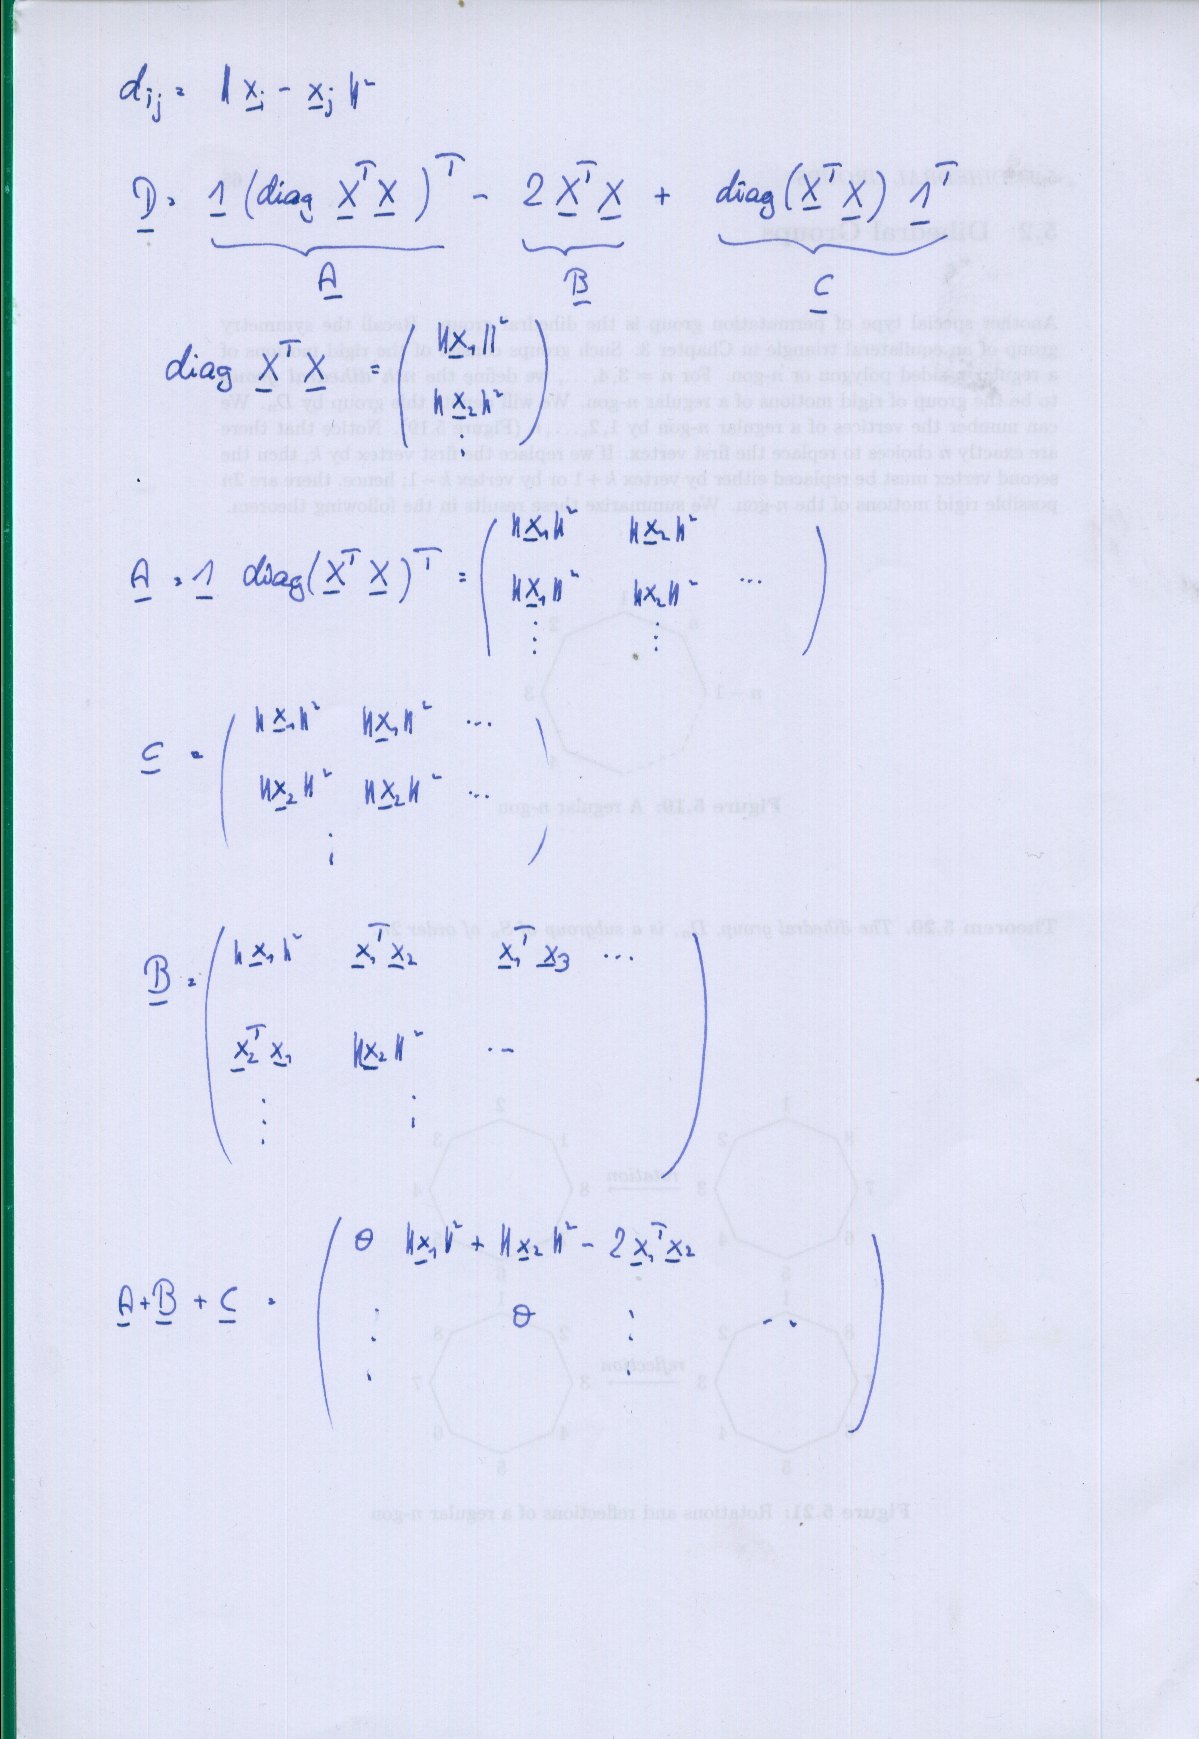
\includegraphics[scale=0.5]{images/edm_0001.png}
\end{figure}

\subsubsection{Derivation of II - B}\label{derivation-of-ii---b}

The n points in a d-dimensional Euclidean space are stored in the
columns of a matrix \(X = [x_1 x_2 \cdots x_n]\).

The edm of this matrix is given by


\begin{equation}
\label{edm_def}
edm(X) = \mathbf{1} \text{diag}(X^T X)^T - 2 X^T X + \text{diag}(X^T X) \mathbf{1}^T
\end{equation}


The task is to reconstruct the matrix X (the points) based on (an
estimate of) the euclidian distance matrix. Later Sections of the paper
deal with noisy and non-complete observations of the EDM but in the
beginning it is assumed that the EDM is fully and correctly known.

The first assumption (leading to (8) etc) is that \(x_1\) lies at the
origin. Then the first part of the EDM expression above becomes
\(\mathbf{1} \text{diag}(X^T X)^T = \mathbf{1} D e_1\) (with \(e_1\)
begin the first unit vector; i.e. \(e_1 = (1 0 \cdots 0)^T\) and
therefore \(D e_1\) selects the first column of D).

Therefore, we can solve the equation above for \(X^T X\) as follows:

\[
X^T X = -\frac{1}{2} \left[ edm(X) - \mathbf{1} d_1^T - d_1 \mathbf{1}^T \right]
\]

We can obtain from \(X^T X\) the matrix \(X\) by performing an
eigenvalue decomposition \(X^T X = U \Lambda U^T\). Then
\(X_{\text{sqrt}} = \sqrt{\Lambda} U^T\) and
\(X_{\text{sqrt}}^T X_{\text{sqrt}} = X^T X\).

Assuming that the eigenvalues are ordered by size, we throw away all but
the first n ones. The esimtated matrix \(X_{\text{est}}\) is then given
by \(X_{\text{est}} = \sqrt{\Lambda} U^T\).

\subsubsection{Uniqueness of EDM}\label{uniqueness-of-edm}

If we rotate and/or shift the point matrix \(X\), the edm should stay
the same. A rotaion is expressed as \(\tilde{X} = QX\), where \(Q\) is
an orthogonal matrix; i.e. \(Q^T Q = I\). In the EDM expression
\(\eqref{edm_def}\), only the term \(X^T X\) appears; considering
\(\tilde{X}\) instead, we have
\(\tilde{X}^T \tilde{X} = X^T Q^T Q X = X^T X\) - a rotation does not
affect the EDM.

In a similar spirit, we can show that a linear translation
\(X_t = X + b 1^T\) leaves the emd intact; i.e. \(edm(X_t) = edm(X)\).
